%% This is an example first chapter.  You should put chapter/appendix that you
%% write into a separate file, and add a line \include{yourfilename} to
%% main.tex, where `yourfilename.tex' is the name of the chapter/appendix file.
%% You can process specific files by typing their names in at the 
%% \files=
%% prompt when you run the file main.tex through LaTeX.
\chapter{GPUs and Parallel Programming Models}


\section{Graphics Processing Units (GPU) Computing}

Conventional central processing units (CPU) are reaching the limits for how high the clock frequencies can go. More and more cores are added on each CPU so as to achieve higher computational throughput. However, physical limitations and limitations on the circuit fabrication make more difficult the improvement of the clock speed of the CPU.

Therefore, the CPU faces the problem of keeping its clock frequency growing and have added more cores to counterbalance this. The other hardware part that is used, the graphical processing units (GPUs), which have always been parallel hardware made for real-time 3D renderings, have evolved into devices that may also be programmed and used for general-purpose computing like scientific computations. Specifically, GPUs can run many threads in parallel that fulfill high computation demand and provide large memory bandwidth to serve parallel memory access requests.

Hence, parallel computing imported a new area called GPGPU, or General-Purpose computation on GPU. The importance of GPGPU technology is to provide heterogeneous computations where applications use both the CPU and GPU. Simply, it can increase the speed of applications with a large amount of data just by using the GPU as a co-processor to CPU to accelerate its general purpose computations that were once only managed by the CPU alone. NVIDIA and ATI have been the main GPU manufacturers with a long list of different models and features. Both of these companies have been producing different platforms that can use parallel computing architectures to utilize the GPU’s stream processors in order to gain more speed-up for any computing process. 

Nowadays, CPU systems are basically multi-core systems. They contain handful of strong cores, each supporting approximately one hardware thread. In contrary, GPU systems are called many-core systems containing many but "lighter" threads. There are two major differences between CPU and GPU threads. First, GPUs have small caches but the context switching between threads is essentially fast so as to overlap memory access latency with useful computations. And second, GPUs achieve high performance when thousands of threads execute in parallel while CPUs need the number of threads per core to be small.\\
\begin{figure}[H]
   \centering
       \includegraphics[width=0.5\textwidth]{gpu}
   \caption{GPU Architecture}
   \label{fig:gpuarch}
\end{figure}

As shown in Figure 2-1, GPU is presented as a set of multiprocessors. Each multiprocessor has its own shared memory and registers. The processors connect with DRAM via an interconnection Network.
\section{NVIDIA's Kepler Architecture}

In an attempt to interpret better the results, it seems necessary to explain the GPU architecture (Kepler GK110 architecture) used in this thesis and especially the GPU model (GTX Force 680) used for the development and the experiments.

NVIDIA’s Kepler architecture introduced to improve mainly 3D graphics quality to gamers. Kepler builds on the foundation first established with NVIDIA's Fermi GPU architecture. This architecture demonstrates higher performance and more efficiency in terms of power consumption compared to Fermi. Kepler provides over 1 TFlop of double precision throughput with greater than 80\% DGEMM efficiency versus 60 ‐ 65\% on the prior Fermi architecture. The first product being introduced based on Kepler architecture is the GeForce GTX 680.The design of this architecture was basically focused on improving power efficiency, delivering up to 3x the performance per watt of Fermi.

 In the design of Kepler introduced a new Streaming Multiprocessor, called “SMX” one of the keys to GeForce GTX 680’s performance. For improved power efficiency, the SMX runs at graphics clock rather than 2x graphics clock, but with 1536 CUDA cores in GK104, the GeForce GTX 680 SMX provides 2x the performance per watt of Fermi’s SM (GF110). This allows the GeForce GTX 680 to deliver higher performance/watt when compared to GeForce GTX 580. The GeForce GTX 680 GPU consists of four Graphics Processing Clusters (GPCs), eight next-generation Streaming Multiprocessors (SMX), and four memory controllers.
 
\begin{figure}[H]
   \centering
       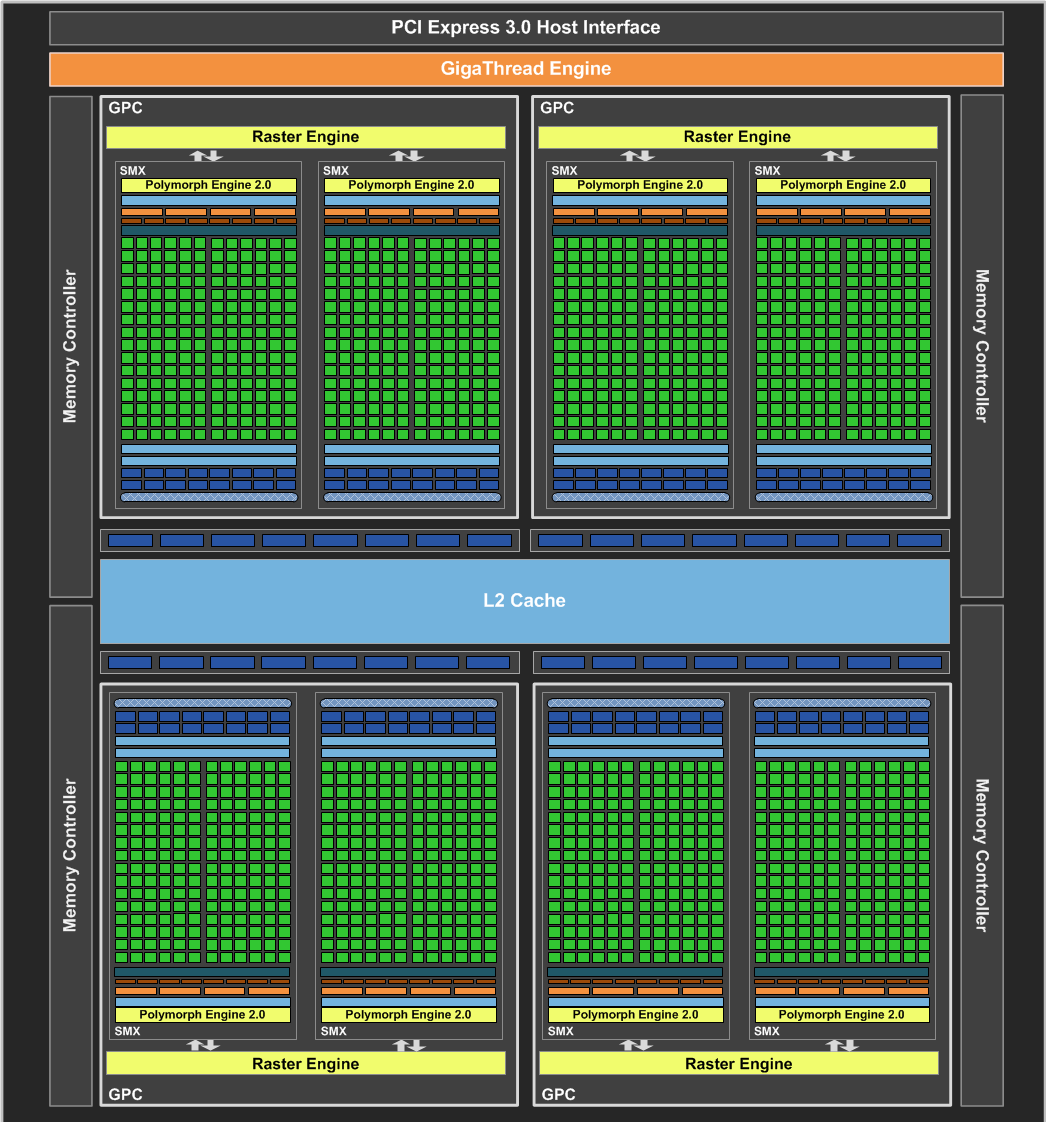
\includegraphics[width=0.5\textwidth]{kepler}
   \caption{Kepler Architecture}
   \label{fig:kepler arch}
\end{figure}

GeForce GTX 680 contains four GPCs, delivering 32 pixels per clock. Each GPC has a dedicated raster engine and two SMX units. With a total of eight SMX units, the GeForce GTX 680 implementation has 1536 CUDA Cores.  GeForce GTX 680’s memory subsystem was also completely revamped, resulting in dramatically higher memory clock speeds. GeForce GTX 680 operates at 6008MHz data rate. Tied to each memory controller are 128KB L2 cache and eight Raster Operations (ROP) units (each of the eight ROP units processes a single color sample). With four memory controllers, a full GeForce GTX 680 GPU has 512KB L2 cache and 32 ROPs (i.e., 32 color samples).

The SM is the heart of NVIDIA’s unified GPU architecture. Most of the key hardware units for graphics processing reside in the SM. The SM’s CUDA cores perform pixel/vertex/geometry shading and physics/compute calculations. Texture units perform texture filtering and load/store units fetch and save data to memory. Special Function Units (SFUs) handle transcendental and graphics interpolation instructions. Finally, the Polymorph Engine handles vertex fetch, tessellation, viewport transform, attribute setup, and stream output. Kepler GK110 supports the CUDA Compute Capability 3.5.

SMX Processing Core Architecture each of the Kepler GK110 SMX units feature 192 single precision CUDA cores, and each core has fully pipelined floating ‐ point and integer arithmetic logic units. Kepler retains the full compliant single and double precision arithmetic introduced in Fermi, including the fused multiply - add (FMA) operation.
The SMX schedules threads in groups of 32 parallel threads called warps. Each SMX features four warp schedulers and eight instruction dispatch units, allowing four warps to be issued and executed concurrently. Kepler’s quad warp scheduler selects four warps, and two independent instructions per warp can be dispatched each cycle.

\begin{figure}[H]
   \centering
       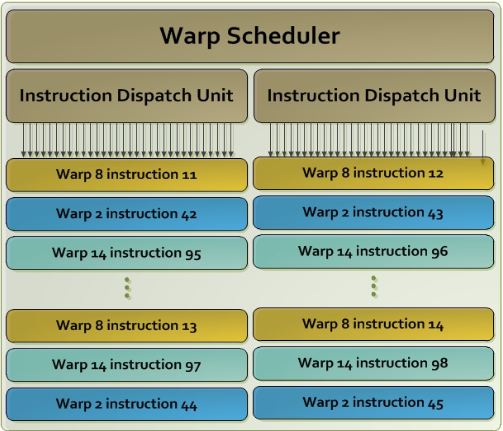
\includegraphics[width=0.5\textwidth]{warp_scheduler}
   \caption{Warp Scheduler}
   \label{fig:warp scheduler}
\end{figure}

To improve performance Kepler introduced a new shuffle instruction, which allows threads within a warp to share data. Previously, sharing data between threads within a warp required separate store and load operations to pass the data through shared memory. With the Shuffle instruction, threads within a warp can read values from other threads in a warp in just about any imaginable permutation. Shuffle supports arbitrary indexed references.
 
In order to increase performance changes have been made in Kepler for the atomic operations. The atomic operations are executed individually from every thread and their execution cannot be interrupted. Atomic operations are widely used in parallel programming in order to succeed synchronization between threads. Throughput of global memory atomic operations on Kepler GK110 is substantially improved compared to the Fermi generation. Atomic operation throughput to a common global memory address is improved by 9x to one operation per clock. Kepler GK110 also expands the native support for 64‐bit atomic operations in global memory. Besides atomicAdd, atomicCAS, and atomicExch, GK110 supports atomicMax, atomicMin, atomicAnd, atomicOr and atomicXor [1].

Kepler keeps a similar memory hierarchy to Fermi. The Kepler architecture supports a unified memory request path for loads and stores, with an L1 cache per SMX multiprocessor. Kepler GK110 also enables compiler directed use of an additional new cache for read‐only data as shown in Figure. As in Fermi architecture in the Kepler GK110 architecture, each SMX has 64 KB of on‐chip memory that can be configured as 48 KB of shared memory with 16 KB of L1 cache, or as 16 KB of shared memory with 48 KB of L1 cache. In Kepler now is permitted a 32KB/32KB split between shared memory and L1 cache, something that offers extra flexibility. To support the increased throughput of each SMX unit, the shared memory bandwidth for 64b and larger load operations is also doubled compared to the Fermi SM, to 256B per core clock.

\begin{figure}[H]
   \centering
       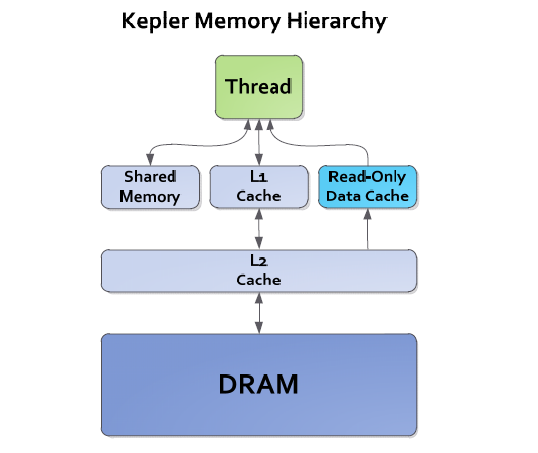
\includegraphics[width=0.5\textwidth]{memory_hieranchy}
   \caption{Kepler Memory Hierarchy}
   \label{fig:memory hieranchy}
\end{figure}

Except from L1 cache, an 48KB cache for data is added that is known to be read‐only for the duration of the function. Another feature met in Kepler GK110 GPU is an improved L2 cache where there are 1536KB of dedicated L2 cache memory, double the amount of L2 available in the Fermi architecture. The L2 cache on Kepler offers up to 2x of the bandwidth per clock available in Fermi. Like Fermi, Kepler’s register files, shared memories, L1 cache, L2 cache and DRAM memory are protected by a Single‐Error Correct Double‐Error Detect (SECDED) ECC code. In addition, the Read‐Only Data Cache supports single - error correction through a parity check; in the event of a parity error, the cache unit automatically invalidates the failed line, forcing a read of the correct data from L2.

\section{NVIDIA CUDA Programming Model}

Compute Unified Device Architecture (CUDA) is a general purpose parallel computing platform and programming model introduced by NVIDIA. CUDA is mostly used to increase the efficiency in the solution of large computational problems in relation to CPU.

CUDA C is an extension of C. Actually CUDA can be considered as C with a few keywords. The programmer defines functions, called kernels. Kernels are executed N times in parallel by N different CUDA threads and only access GPU memory. A kernel can be defined with the \_\_global\_\_ declaration specifier when launched from CPU. A kernel may be launched from another kernel using the \_\_device\_\_ declaration specifier. The programmer is able to define the number of CUDA threads that execute the kernel using the <<<…>>> execution configuration syntax. At each thread that executes the kernel is assigned a unique thread ID that can be referred to via the threadIdx variable. Threads are managed in groups of 32, called warps. Instructions are issued per warp. If an operand is not ready the warp will stall. Computations can be performed in one, two and three-dimensions. For that purpose, threadIdx is a 3-component vector (threadIdx.x, threadIdx.y, threadIdx.z). This provides a natural way to invoke computation across the elements in a domain such as a vector, matrix, or volume. The number of threads per block is limited, due to limited memory resources of the processor core, on which all threads per block within the block reside. In most cases the number of threads per block reflects the problem geometry. On current GPUs, threads per block are up to 1024 threads. 

Blocks do not migrate among processors, execute on one multiprocessor. Several blocks can execute concurrently on one multiprocessor. They are organized into a one, two, or three-dimensional grid of thread blocks as illustrated by Figure 2-5. The number of thread blocks in the grid usually results from the amount of data to be processed to the number of threads per block. 

\begin{figure}[H]
   \centering
       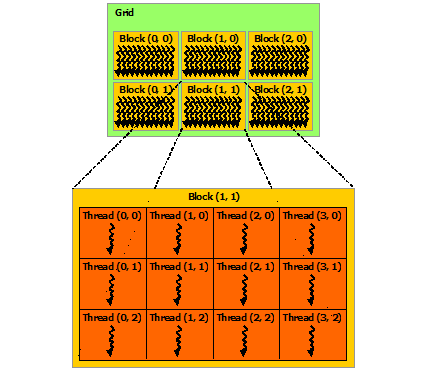
\includegraphics[width=0.5\textwidth]{blocks}
   \caption{Cuda Blocks}
   \label{fig:Blocks}
\end{figure}

In correspondence with the threads in the blocks, each block within the grid can be identified by a one, two, or three-dimensional index accessible within the kernel through the built-in blockIdx variable. The dimension of the thread block can be accessed within the kernel through the built-in blockDim variable. 

Every thread has private local memory. Each thread block has shared memory visible to all threads of the block and with the same lifetime as the block. Shared memory is used by threads to contribute for shared data and synchronize their execution to avoid simultaneous memory accesses. In particular, by calling the \_\_syncthreads() function threads can succeed synchronization.  \_\_syncthreads() is a barrier where all threads in a block must wait before any is allowed to proceed. All threads have access to the same global memory. The constant and texture memory spaces are two additional read-only memory spaces accessible by all threads. The global, constant, and texture memory spaces are persistent across kernel launches by the same application. 


In correspondence with the threads in the blocks, each block within the grid can be identified by a one-dimensional, two-dimensional, or three-dimensional index accessible within the kernel through the built-in blockIdx variable. The dimension of the thread block can be accessed within the kernel through the built-in blockDim variable. Every thread has private local memory. Each thread block has shared memory visible to all threads of the block and with the same lifetime as the block. Shared memory is used from threads to cooperate, share data and synchronize their execution to avoid simultaneous memory accesses. In particular, by calling the \_\_syncthreads() function threads can succeed  synchronization. \_\_syncthreads() is a barrier where all threads in a block must wait before any is allowed to proceed. All threads have access to the same global memory. The constant and texture memory spaces are two additional read-only memory spaces accessible by all threads. The global, constant, and texture memory spaces are persistent across kernel launches by the same application ([2], [3], [4]). 

\begin{figure}[H]
   \centering
       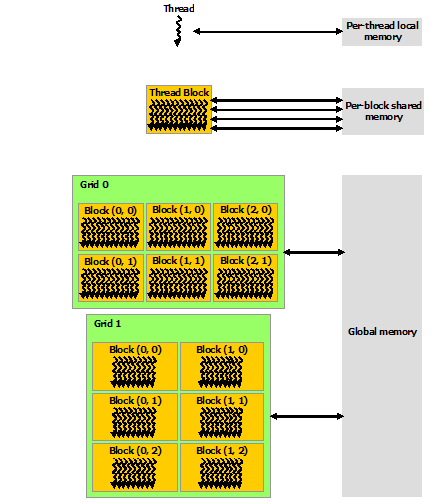
\includegraphics[width=0.5\textwidth]{grids}
   \caption{Cuda Grids}
   \label{fig:Grids}
\end{figure}

The CUDA programming model assumes a system composed of a host and a device, each with their own separate memory. Serial code executes in a host (CPU) thread. Parallel code executes in many device (GPU) threads across multiple processing elements. Device memory is typically allocated using cudaMalloc() and freed using cudaFree() and data transfer between host memory and device memory are typically done using cudaMemcpy(). 

Here are some examples of typical instructions:\\
Kernel definition example:
\begin{lstlisting}[frame=single]
__global__ void kernel( int *a, int dimx, int dimy ){
	inttx = blockIdx.x * blockDim.x + threadIdx.x;
	intty = blockIdx.y * blockDim.y + threadIdx.y;
	intidx = ty*dimx + tx;
	a[idx] = a[idx]+1;
}
\end{lstlisting}
Kernel launch example:
\begin{lstlisting}[frame=single]
int *d_a = 0;
cudaMalloc ( (void**)&d_a, num_bytes );
dim3 grid, block;
block.x = 4;
block.y = 4;
grid.x = dimx / block.x;
grid.y = dimy / block.y;
kernel<<<grid, block>>>( d_a, dimx, dimy );
\end{lstlisting}